\section{数值实验与交叉验证}

本章通过系统的数值实验验证所构建的 SOCP 轨迹优化问题在多个独立求解器框架下的一致性，评估各求解器的计算性能，并分析单精度浮点数在该问题上的适用性限界。

\subsection{实验设置}

所有实验在以下硬件平台上执行：Intel N150 处理器（LattePanda Iota 开发板，4 核 4 线程，最高睿频 3.4 GHz，TDP 仅 6 W），8 GB LPDDR5 内存，运行 Ubuntu 24.04 LTS 操作系统。该平台兼具 x86 桌面级性能与嵌入式低功耗特征，适合验证算法在资源受限环境中的部署可行性。所有计时测试均关闭 CPU 频率缩放和睿频功能以降低测量方差。

软件环境方面，SOCP 求解器采用 ECOS 2.0.10~\cite{domahidi2013ecos}（纯 C 实现，含 AVX 加速版与标量版两个编译目标）和 Clarabel 0.11（Rust 实现，通过 Python 接口调用）。NLP 求解器采用 IPOPT 3.14~\cite{wachter2006implementation}（通过 CasADi 3.6~\cite{andersson2019casadi} 接口调用）。CVXPY 1.x~\cite{diamond2016cvxpy} 作为高阶建模层为 ECOS 和 Clarabel 提供统一的 SOCP 描述语言。C 代码使用 GCC 13.3 编译，优化选项为 \texttt{-O3 -march=native}。C 手写版通过 CMake 构建系统配置三个编译目标：\texttt{ecos\_avx}（开启 \texttt{-mavx -mfma}）、\texttt{ecos\_scalar}（纯标量指令）、\texttt{ecos\_auto}（CasADi 自动生成矩阵数据）。

所有求解器的收敛容差配置如表 \ref{tab:solver_config} 所示。ECOS 采用原对偶内点法求解 SOCP 标准形式，本实验设置绝对容差 \texttt{abstol} = $1\times10^{-8}$，相对容差 \texttt{reltol} = $1\times10^{-8}$，最大迭代次数 100。Clarabel 同样基于原对偶内点法求解 SOCP，使用默认收敛容差（\texttt{tol\_gap\_abs} = $1\times10^{-8}$，\texttt{tol\_feas} = $1\times10^{-8}$）。IPOPT 无法直接处理二阶锥约束，因此采用第 3 章所述的光滑等价形式——将 $\|x\|\leq t$ 替换为 $t^2 - x^\top x \geq 0$ 且 $t \geq 0$——将 SOCP 转化为 NLP 后由 IPOPT 的原对偶内点滤线搜索算法求解，收敛容差 \texttt{tol} = $1\times10^{-8}$。

\begin{table}[tbp]
\centering
\caption{求解器配置对比}
\label{tab:solver_config}
\begin{tabular}{clll}
\toprule
求解器 & 问题类型 & 算法 & 收敛容差 \\
\midrule
ECOS       & SOCP & 原对偶内点法 & \texttt{abstol}=$1\times10^{-8}$ \\
Clarabel   & SOCP & 原对偶内点法 & 默认（$1\times10^{-8}$） \\
IPOPT      & NLP（光滑等价） & 内点滤线搜索 & \texttt{tol}=$1\times10^{-8}$ \\
\bottomrule
\end{tabular}
\end{table}

三款求解器在记录中扮演不同角色：ECOS 提供 C 原生 SOCP 接口并用于当前可执行目标；Clarabel 提供另一条 SOCP 数值路径和单精度对比平台；IPOPT 作为通用 NLP 求解器，提供光滑约束形式的历史 comparison 记录。Clarabel 与 IPOPT 条目当前是静态记录，不由 quick CI 动态重跑，也不单独用于判定凸化是否无损。

\subsection{最优轨迹分析}

通过 CVXPY+ECOS 求解器获得的最优轨迹涵盖了着陆器从初始状态到终端着陆的完整运动过程。

\begin{figure}[tbp]
\centering
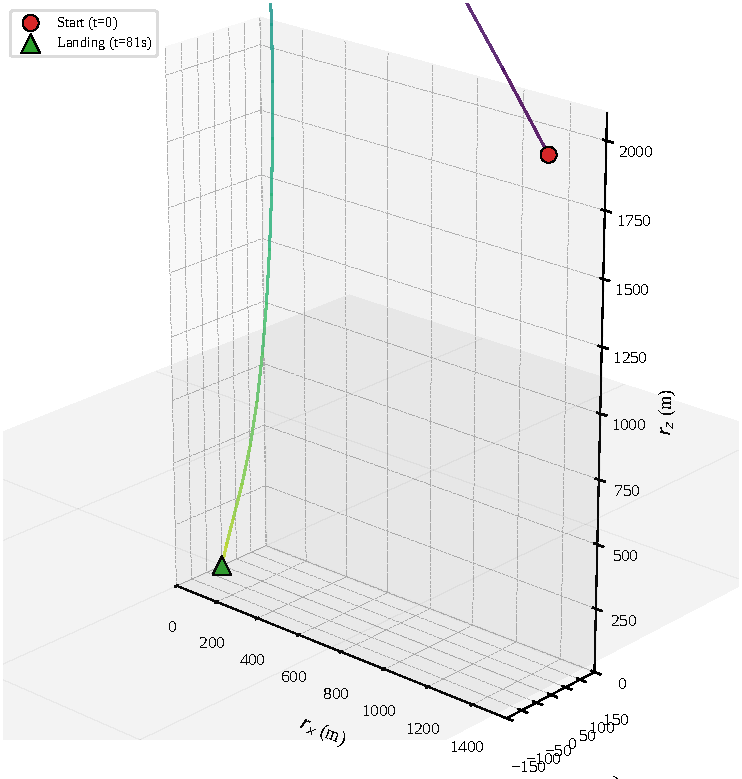
\includegraphics[width=\mediumfig]{figures/fig01_3d_trajectory.pdf}
\caption{三维着陆轨迹。起始于$(1500,0,2000)$ m，终止于原点。}
\label{fig:3d_trajectory}
\end{figure}

图 \ref{fig:3d_trajectory} 展示了着陆器在三维空间中的下降轨迹，起始于 $(1500, 0, 2000)$ m，三维路径平滑收敛至原点。轨迹在水平面（$yz$ 平面）的投影近乎是一条直线，表明最优解倾向于沿最短水平路径指向着陆点。图 \ref{fig:position_time} 给出了三轴位置随时间的变化曲线：$r_x$ 从 1500 m 单调递减至零，呈平滑抛物线外形——在前半段斜率较缓（接近零），在约 $t=30$ s 后斜率明显增大再逐渐归零；$r_y$ 始终维持在零附近，表明轨迹优化在水平 $y$ 方向几乎不产生机动，这与初始 $v_y = 0$ 且目标 $r_y=0$ 的对称边界条件一致；$r_z$ 从 2000 m 均匀下降至零，在终端附近斜率趋缓。该轨迹特征直观反映了下滑角锥约束对 $r_x$ 和 $r_z$ 之间比例关系的限制——$r_z$ 被约束在以 $r_x\tan\theta$ 为半径的锥体内，其中 $\theta = 86^{\circ}$，轨迹接近垂直下降。

\begin{figure}[tbp]
\centering
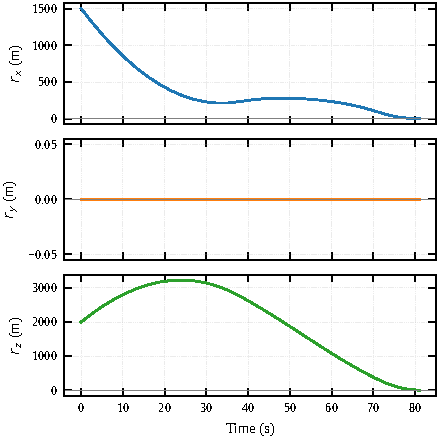
\includegraphics[width=\widefig]{figures/fig02_position_time.pdf}
\caption{非零位置分量时间曲线。上：$r_x$；下：$r_z$；对称边界使 $r_y$ 全程为零。}
\label{fig:position_time}
\end{figure}

图 \ref{fig:velocity_time} 显示速度分量的演化过程。$v_x$ 从初始的 -75 m/s 逐渐收敛至零，下降初期经历约 20 s 的加速段（负向速度绝对值从 75 增大至约 95 m/s），其后进入稳定减速段并在终端时刻归零。$v_x$ 先加速后减速的行为与最优燃料控制中典型的"先加速后减速"特征一致：在着陆前期，利用重力将势能转化为动能以提高发动机效率，在后期集中消耗燃料进行快速减速。$v_z$ 从 100 m/s 持续递减至零，减速过程贯穿整个 81 s 飞行时段，没有出现加速段——这是因为 $v_z$ 方向与重力方向垂直，不受重力助推作用。$v_y$ 始终为极小值（量级 $10^{-6}$ m/s）。速度剖面表明，着陆器的减速机动主要由推力在三轴上的分量配合实现，其中 $v_z$ 的衰减消耗了最大量的控制能量。

\begin{figure}[tbp]
\centering
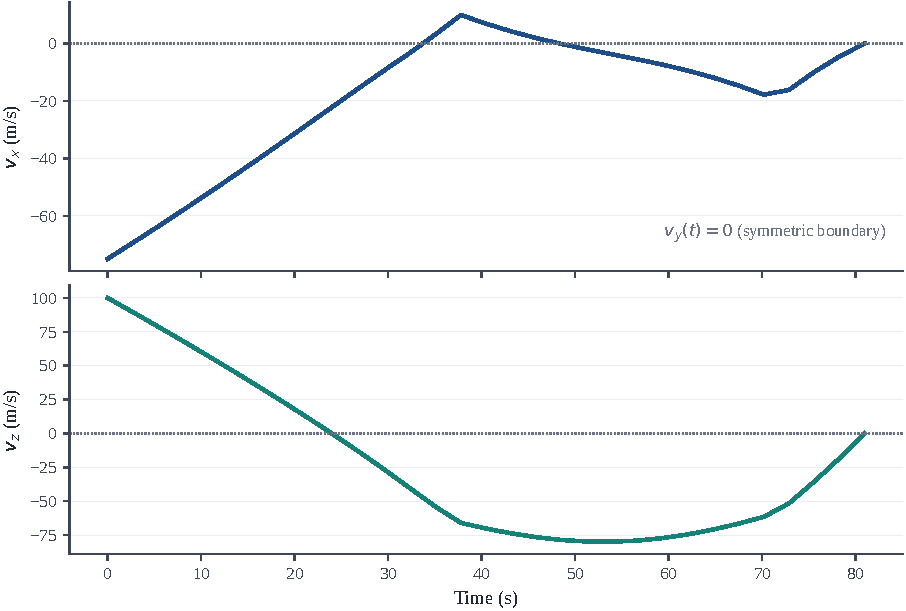
\includegraphics[width=\widefig]{figures/fig03_velocity_time.pdf}
\caption{非零速度分量时间曲线。上：$v_x$；下：$v_z$；对称边界使 $v_y$ 全程为零。}
\label{fig:velocity_time}
\end{figure}

图 \ref{fig:mass_evolution} 展示了当前标称数值解中着陆器质量从初始 1905.0 kg 至终端 1504.272 kg 的单调递减过程，对应目标值 400.728 kg（按一位小数记为 400.7 kg）。独立解审计同时发现，该终端质量低于 1505 kg 干重下界约 0.728 kg；因此 400.7 kg 只能作为各实现数值一致性的回归基准，不能表述为已满足全部物理约束的确认性燃料结果。质量曲线的斜率在大部分飞行时间内近乎恒定，仅在终端最后三步略有缓减，这描述了当前数值解的推力使用特征，但不消除上述干重违反。

\begin{figure}[tbp]
\centering
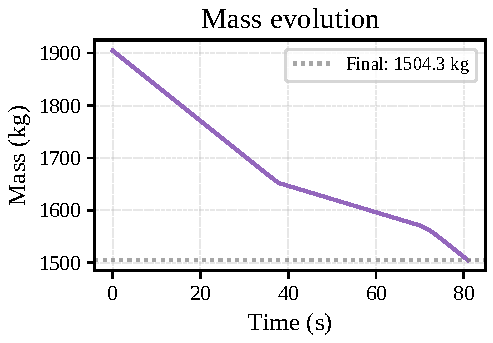
\includegraphics[width=\widefig]{figures/fig04_mass_evolution.pdf}
\caption{当前标称数值解的质量变化曲线。终端质量 1504.272 kg，低于 1505 kg 干重下界约 0.728 kg。}
\label{fig:mass_evolution}
\end{figure}

图 \ref{fig:thrust_comparison} 展示当前标称数值解中的推力幅值 $\|u\|$、松弛变量 $\sigma$ 与质量相关的推力上界。在绘图精度下，$\|u\|$ 与 $\sigma$ 在大部分控制区间接近，并在部分区间逼近上界。这可作为松弛间隙的数值诊断线索，但不能单独确认原非凸问题与 SOCP 的等价性~\cite{acikmese2013,acikmese2007lossless}。终端数步内推力幅值下降，记录峰值约为 8.66 N/kg。由于同一标称解存在干重下界违反，这些曲线只描述当前数值输出，不构成完整物理可行性结论。

\begin{figure}[tbp]
\centering
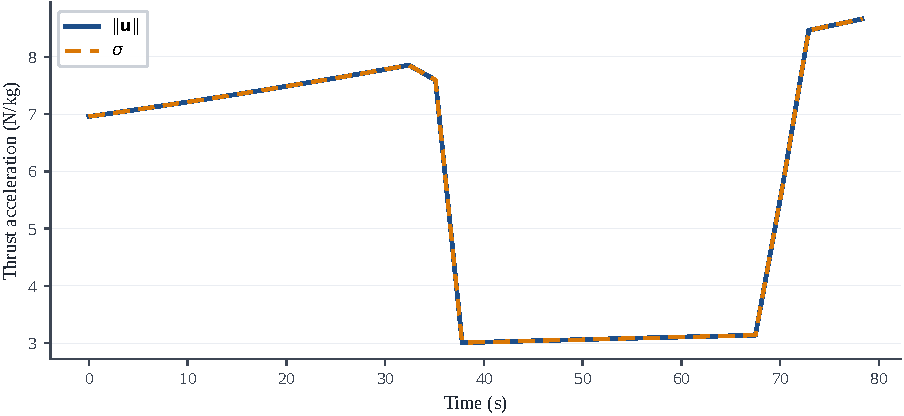
\includegraphics[width=\widefig]{figures/fig05_thrust_comparison.pdf}
\caption{当前标称数值解的推力幅值 $\|\bm{u}\|$ 与松弛变量 $\sigma$；二者的数值间隙用于诊断，不作为凸化无损性的独立证明。}
\label{fig:thrust_comparison}
\end{figure}

图 \ref{fig:glide_slope} 验证了下滑角约束的满足情况。上子图显示 $[r_y, r_z]$ 向量的范数与 $r_x\tan\theta$ 的关系，二者始终保持接触或分离；下子图给出了余量（$r_x\tan\theta - \|[r_y,r_z]\|$），该余量始终非负（$r_x\tan\theta \geq \|[y,z]\|$），在轨迹中段约束最为紧凑（余量在 $t=40$--60 s 区间接近零），说明下滑角约束在最优轨道的某些时刻确实起到了限制作用。特别值得注意的是，余量在全程均不严格为零但在轨迹中段逼近零，这表明下滑角约束对最优解施加了有效影响但并未全程激活——最优解在中段因物理条件自然趋近锥边界。

\begin{figure}[tbp]
\centering
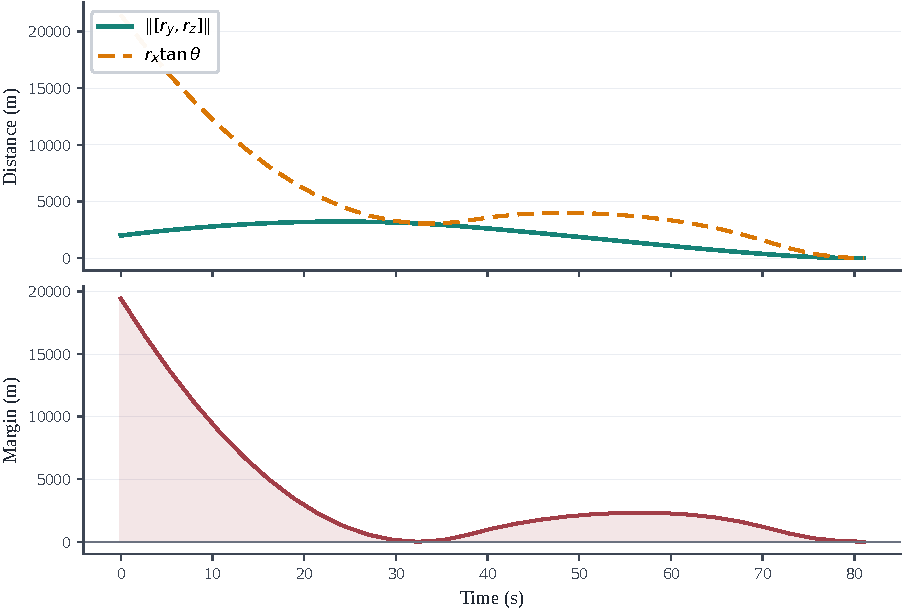
\includegraphics[width=\widefig]{figures/fig06_glide_slope.pdf}
\caption{下滑角约束验证。上：$\|[r_y,r_z]\|$ 与 $r_x\tan\theta$ 对比；下：约束余量。}
\label{fig:glide_slope}
\end{figure}

图 \ref{fig:thrust_cone} 验证了每个实际控制区间上的推力锥关系。上图中 $\sigma$ 与 $\|u\|$ 在视觉上重合；下图将其差值以科学计数法放大后显示，数值残差处于 $10^{-9}$ N/kg 量级，属于求解容差范围。终端节点不对应一个施加的控制区间，故未纳入该图的控制量比较。

\begin{figure}[tbp]
\centering
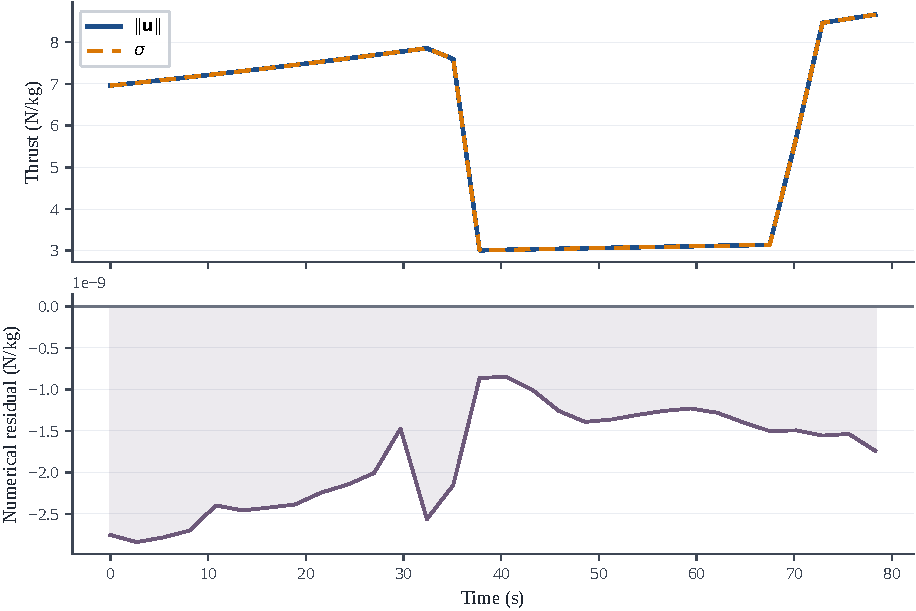
\includegraphics[width=\widefig]{figures/fig07_thrust_cone.pdf}
\caption{推力锥约束验证。上：实际控制区间上的 $\|\bm{u}\|$ 与 $\sigma$ 对比；下：数值残差 $\sigma - \|\bm{u}\|$。}
\label{fig:thrust_cone}
\end{figure}

\subsection{交叉验证}

\subsection{物理修正的自由终端时间与网格审计}

为避免把历史 $t_f=81$ s 手写基线的干重违反误读为物理可行结果，本文另建了物理修正的参数化研究模型（版本由 manifest 固定）。它在每个节点显式施加 $m\geq1505$ kg，并在每个控制区间的九个内部采样点施加下滑角 SOC 约束；固定 $(N,t_f)$ 的内层仍为 SOCP，终端时间由版本化 Decimal 网格外层搜索。该模型不修改、生成或替代 \texttt{MarsLanding/MarsLanding.c}；后者始终是 $N=30,t_f=81$ s 的原始、独立人工手写 CRS--CCS 参考实现。

图 \ref{fig:free_time_mesh} 从 75 条原始记录重算而来。N=20 的 15 个 ECOS 候选均明确不可行。N=30、40、60 分别得到最优已审计 ECOS 候选 $(t_f,\mathrm{fuel})=(78.02\,\mathrm{s},399.8010\,\mathrm{kg})$、$(78.02\,\mathrm{s},399.3954\,\mathrm{kg})$ 和 $(77.98\,\mathrm{s},398.9147\,\mathrm{kg})$。N=60 对应的 Clarabel 复算为 $398.9146$ kg，燃料差约 $2.1\times10^{-5}$ kg，且通过预注册审计。N=30、40 的 Clarabel 点分别因推力锥/包络残差略超过 $10^{-6}$ 门槛而被归为 \texttt{physical\_violation}；它们不能作为双求解器确认点。

\begin{figure}[tbp]
\centering
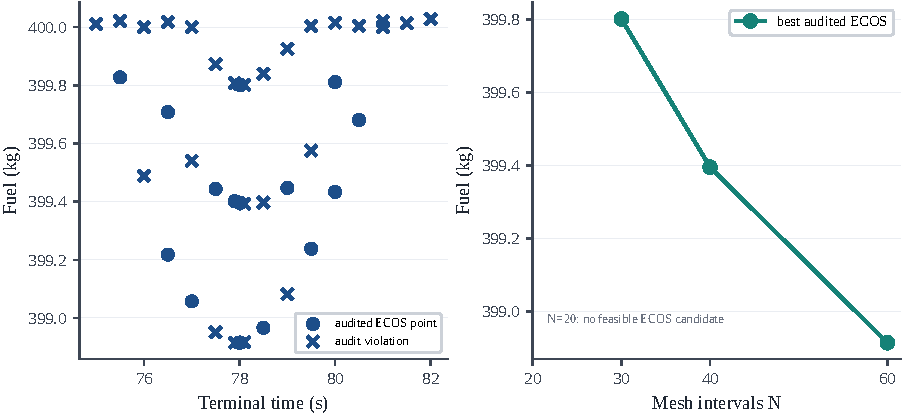
\includegraphics[width=\widefig]{figures/fig11_free_time_mesh.pdf}
\caption{物理修正自由终端时间研究。左：ECOS 候选的燃料--时间关系及分类；右：每个网格独立搜索得到的最佳已审计 ECOS 点。N=20 无可行点，且 N=30--60 的燃料仍随网格变化，故不能宣称连续时间最优或网格收敛。}
\label{fig:free_time_mesh}
\end{figure}

这项证据纠正了早期约 $399.733$ kg 的探索值：其节点约束虽可满足，但独立密集区间审计曾发现约 27.2 m 的下滑锥违反。加入区间 SOC 约束后，该数字不再可用。当前四网格数据也尚未满足连续三网格的预注册收敛阈值；它证明了模型缺陷被发现和修正，而不是已经完成连续时间最优性证明。

表 \ref{tab:cross_validation} 汇总仓库当前记录的六条数值路径，但其证据分为两个边界明确的集合。第一组是可由构建产物直接复核的三个 C ECOS 路径：手写矩阵 AVX 版、手写矩阵标量版和自动生成矩阵版。第二组是 \texttt{solver\_comparison.json} 中保存的三条 Python 路径：CVXPY+ECOS、CVXPY+Clarabel 和 CasADi+IPOPT。前两条 Python 路径求解 SOCP，IPOPT 使用 NLP 光滑等价形式。该表只陈述这些记录在燃料目标值上的数值一致性，不表示六条路径均由 quick CI 动态重跑，也不表示它们已通过全部物理残差审计。

\begin{table}[tbp]
\centering
\caption{六条求解路径的记录值及其数值对比}
\label{tab:cross_validation}
\begin{tabular}{lclrr}
\toprule
求解方案 & 问题类型 & 建模方式 & 燃料消耗 (kg) & 偏差 (\%) \\
\midrule
ECOS AVX（C 手写） & SOCP & 手写稀疏 CCS 矩阵 & 400.7 & 基准 \\
ECOS 标量（C 手写） & SOCP & 手写稀疏 CCS 矩阵 & 400.7 & 0.0 \\
ECOS（C 自动生成） & SOCP & CasADi 生成 CCS 矩阵 & 400.7 & 0.0 \\
CVXPY+ECOS & SOCP & CVXPY 高阶建模 & 400.7 & 0.0 \\
CVXPY+Clarabel & SOCP & CVXPY 高阶建模 & 400.7 & 0.0 \\
CasADi+IPOPT & NLP & 光滑等价 SOC $\to$ NLP & 400.7 & 0.0 \\
\bottomrule
\end{tabular}
\end{table}

三个 C 可执行路径当前均报告 400.7 kg；Python comparison 文件中的三条记录也均为 400.7 kg。这里的 0.0\% 是按一位小数记录后的目标值差异，不应解读为高精度逐位相等。尤其是，这一一致性不消除前述标称解约 0.728 kg 的干重下界违反。

\begin{figure}[tbp]
\centering
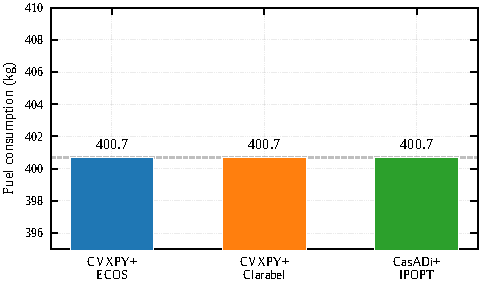
\includegraphics[width=\widefig]{figures/fig08_fuel_comparison.pdf}
\caption{Python comparison 文件中的三条燃料目标值记录；按一位小数均为 400.7 kg。}
\label{fig:fuel_comparison}
\end{figure}

这两个证据集合为实现一致性提供了交叉检查，但不足以单独证明算法或物理模型正确。C 手写版与自动生成版保持独立：前者以 CRS\_PUSH 宏逐行组装并转换为 CCS，后者使用 CasADi 生成的 CCS 数据；CVXPY 则通过约束表达式规范化生成问题。它们得到相同的一位小数目标值，可以发现明显的装配或符号回归，但不能排除小于显示精度的差异，也不能替代约束残差审计。

Python comparison 中 ECOS 与 Clarabel 的记录值一致，说明该数据快照没有显示求解器级别的一位小数偏差。由于 quick CI 不动态运行 Clarabel 或 IPOPT，这一结论严格限于版本库中的 comparison 文件；环境、依赖或模型变化后必须重新生成证据，不能由静态快照外推。

CasADi+IPOPT 的记录值与 SOCP 路径相同，可作为光滑 NLP 路径的历史数值对照；但静态记录本身不能构成无损凸化等价性的最终确认。该判断还需要可重放的求解输出、锥松弛间隙和全部物理约束残差共同支持~\cite{acikmese2013}。

需要特别指出的是，IPOPT 版本使用光滑等价形式（$t^2 - x^\top x \geq 0$）替代二阶锥约束。该转换要求在 $t \geq 0$ 条件下确保 $t^2 - x^\top x \geq 0$ 与原锥约束 $\|x\|\leq t$ 完全等价。曾在实验早期尝试将 SOC 约束错误地拆分为标量不等式 $r_x \geq 0$、$r_y \geq 0$、$r_z \geq 0$，结果导致燃料消耗偏差高达 23\%，因为该拆分完全丢失了范数约束的耦合关系，仅限制了位置符号而未约束其范数。这一教训再次强调了锥约束作为整体处理的必要性。

\subsection{计算性能分析}

求解时间是评估部署可行性的一个指标，但必须限定计时范围和运行环境。火星着陆动力下降段持续时间约 60--90 s，制导重规划常以 1--10 Hz 为设计参考。表 \ref{tab:performance} 汇总五条现有计时记录；C 路径统计预初始化后 1000 次重复 \texttt{ECOS\_solve} 的平均 CPU 时间，Python 条目则包含各自记录路径的上层调用开销，因此两组数值不属于严格同口径端到端基准。

\begin{table}[tbp]
\centering
\caption{计算性能对比（1000 次重复测量均值）}
\label{tab:performance}
\begin{tabular}{lrc}
\toprule
求解方案 & 单次求解耗时 (ms) & 相对基准 \\
\midrule
ECOS AVX（C 手写，冻结均值） & 7.361 & 限定均值 \\
CVXPY+ECOS & 372.22 & $\times$46.5 \\
CVXPY+Clarabel & 348.06 & $\times$43.5 \\
CasADi+IPOPT & 5835.4 & $\times$729 \\
\bottomrule
\end{tabular}
\end{table}

冻结报告中的 C 手写 AVX 目标均值为 7.361 ms/次。该值由 \texttt{clock()} 累计 setup 后 1000 次 \texttt{ECOS\_solve} 的 CPU 时间得到；没有逐次 raw samples，不能据此报告 p99、最大值或 WCET，也不是端到端重规划延迟。

\begin{figure}[tbp]
\centering
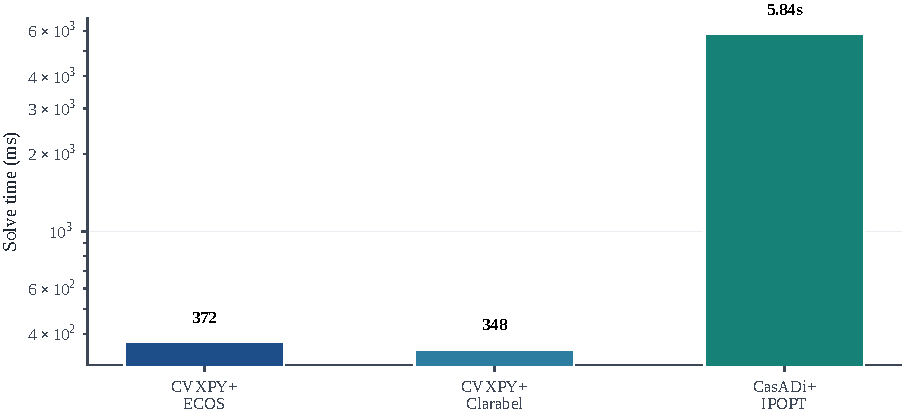
\includegraphics[width=\widefig]{figures/fig09_time_comparison.pdf}
\caption{三种 Python 求解路径的单次求解耗时对比（对数坐标）。}
\label{fig:time_comparison}
\end{figure}先前标量与 AVX/FMA 构建约 2.4\% 的差异没有冻结 raw timing 或硬件计数器支持，现仅保留为待复现实验，不作 SIMD 因果结论。

CVXPY 建模层的引入使测得时间从约 8 ms 增至约 350--370 ms（约 45 倍）。这一差距表明，对小规模 SOCP，建模、规范化和结果回提取会显著影响端到端 Python 调用时间。CVXPY 的调用路径包括约束表达式构造、DCP 分析、规范化、稀疏矩阵组装、求解器调用和结果回提取；该开销适合离线设计，但不宜直接用于星上实时制导。CasADi+IPOPT 耗时约 5.8 s，是三类方案中最慢者，主要因为 NLP 迭代需要反复评估 Jacobian 和 Hessian 矩阵，更适合地面离线校核。

在 SOCP 求解器层面，Clarabel（348 ms）相比 ECOS（372 ms）在 CVXPY 环境下快约 6.5\%。Clarabel 作为 Rust 实现的新型内点法求解器，其 LDL 分解采用了更加缓存友好的超节点（supernodal）策略，减少了内存引用局部性差的间接索引次数。然而，当脱离 CVXPY 建模层并在预初始化工作区上重复调用时，ECOS 的 C 原生接口仍表现出明显优势（约 8 ms）。手写问题数据采用栈上定长数组；ECOS 工作区本身仍由 \texttt{ECOS\_setup()} 分配，硬实时部署需进一步采用静态内存池改造。

\subsection{单精度与双精度对比}

不同嵌入式处理器对单精度和双精度的硬件支持差异较大，具体代价必须以芯片手册和目标构建测量为准。本文仅比较仓库中两组 Clarabel 配置的记录结果，不将其直接外推到硬件选型。

现有记录中，\texttt{Clarabel f32} 使用放宽至 $10^{-6}$ 的容差，\texttt{Clarabel f64} 使用默认配置。由于精度和容差同时变化，这不是控制变量实验。

\begin{figure}[tbp]
\centering
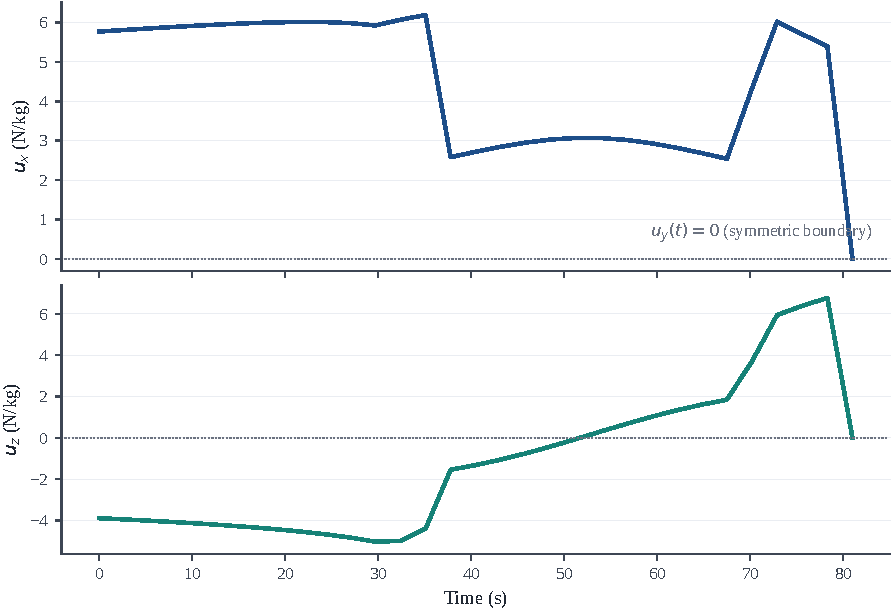
\includegraphics[width=\widefig]{figures/fig10_control_time.pdf}
\caption{非零控制加速度分量 $u_x$、$u_z$ 的时间演化曲线；对称边界使 $u_y$ 全程为零。}
\label{fig:control_time}
\end{figure}

两组不同配置分别记录 1880+ kg 和 400.7 kg，名义差异约 375\%。该观测不能单独归因于浮点精度，也不能在缺少同容差残差审计时断言 KKT 系统崩溃。分离精度影响需要统一模型、容差、缩放、停止条件和审计指标。

变量量级从位置约 $10^3$ m 到 $\exp(-z)$ 约 $5\times10^{-4}$，提示缩放和条件数可能影响数值行为，但这只是诊断假设。另一个可直接计算的局部关系是 $m=\exp(z)$ 下 $dm/dz=m$：在本问题质量约 1500 kg 时，给定的 $z$ 误差会在一阶换算中乘以约 1500。该关系只是局部误差单位换算，不说明自动微分、梯度或 Hessian 被放大同样倍数，也不能解释两组 Clarabel 配置的全部差异。后续应在统一容差下分别测试缩放、精度和残差。

\subsection{蒙特卡洛鲁棒性分析}

先前无冻结数据支持的 Monte Carlo 数字已撤回。现已按 canonical manifest 完成并冻结 1000 个逐样本记录；求解器状态与物理审计分类保持分离。

后续确认实验采用仓库中的 canonical manifest \texttt{near\_nominal\_v1.json}：随机种子固定为 42，计划样本数为 1000；标称初始条件为 $r_0=(1500,0,2000)$ m、$v_0=(-75,0,100)$ m/s；仅对 $r_x,r_z$ 施加半宽 200 m 的均匀增量扰动，仅对 $v_x,v_z$ 施加半宽 20 m/s 的均匀增量扰动，两个 $y$ 分量保持不变。每个样本均由 CVXPY+ECOS 求解，并保存输入、求解器状态、耗时、manifest 摘要和审计指标。

1000 个尝试中，483 个为 \texttt{success}，363 个为 \texttt{physical\_\allowbreak violation}，153 个为 \texttt{solver\_\allowbreak infeasible}，1 个为 \texttt{solver\_error}。审计成功率为 0.483，Wilson 95\% 区间为 $[0.4522,0.5140]$。仅对 483 个成功样本计算的燃料条件分布为：均值 383.8378 kg、样本标准差 9.5240 kg、最小值 360.2158 kg、最大值 399.9547 kg。该条件统计不包含失败样本，不能表述为总体燃料分布或鲁棒性通过。单个 \texttt{solver\_error} 尚未归因，需结合原始记录后续调查。
